%%%%%%%%%%%%%%%%%%%%%%%%%%%%%%%%%%%%%%%%%12pt: grandezza carattere
                                        %a4paper: formato a4
                                        %openright: apre i capitoli a destra
                                        %twoside: serve per fare un
                                        %   documento fronteretro
                                        %report: stile tesi (oppure book)
\documentclass[12pt,a4paper,openright,twoside]{report}
%
%%%%%%%%%%%%%%%%%%%%%%%%%%%%%%%%%%%%%%%%%libreria per scrivere in italiano
\usepackage[italian]{babel}
%
%%%%%%%%%%%%%%%%%%%%%%%%%%%%%%%%%%%%%%%%%libreria per accettare i caratteri
                                        %   digitati da tastiera come � �
                                        %   si pu� usare anche
                                        %   \usepackage[T1]{fontenc}
                                        %   per� con questa libreria
                                        %   il tempo di compilazione
                                        %   aumenta
\usepackage[latin1]{inputenc}
%
%%%%%%%%%%%%%%%%%%%%%%%%%%%%%%%%%%%%%%%%%libreria per impostare il documento
\usepackage{fancyhdr}
%
%%%%%%%%%%%%%%%%%%%%%%%%%%%%%%%%%%%%%%%%%libreria per avere l'indentazione
%%%%%%%%%%%%%%%%%%%%%%%%%%%%%%%%%%%%%%%%%   all'inizio dei capitoli, ...
\usepackage{indentfirst}
%
%%%%%%%%%libreria per mostrare le etichette
%\usepackage{showkeys}
%
%%%%%%%%%%%%%%%%%%%%%%%%%%%%%%%%%%%%%%%%%libreria per inserire grafici
\usepackage{graphicx}
%
%%%%%%%%%%%%%%%%%%%%%%%%%%%%%%%%%%%%%%%%%libreria per utilizzare font
                                        %   particolari ad esempio
                                        %   \textsc{}
\usepackage{newlfont}
%
%%%%%%%%%%%%%%%%%%%%%%%%%%%%%%%%%%%%%%%%%librerie matematiche
\usepackage{amssymb}
\usepackage{amsmath}
\usepackage{latexsym}
\usepackage{amsthm}
%
\oddsidemargin=30pt \evensidemargin=20pt%impostano i margini
\hyphenation{sil-la-ba-zio-ne pa-ren-te-si}%serve per la sillabazione: tra parentesi
					   %vanno inserite come nell'esempio le parole
%					   %che latex non riesce a tagliare nel modo giusto andando a capo.

%
%%%%%%%%%%%%%%%%%%%%%%%%%%%%%%%%%%%%%%%%%comandi per l'impostazione
                                        %   della pagina, vedi il manuale
                                        %   della libreria fancyhdr
                                        %   per ulteriori delucidazioni
\pagestyle{fancy}\addtolength{\headwidth}{20pt}
\renewcommand{\chaptermark}[1]{\markboth{\thechapter.\ #1}{}}
\renewcommand{\sectionmark}[1]{\markright{\thesection \ #1}{}}
\rhead[\fancyplain{}{\bfseries\leftmark}]{\fancyplain{}{\bfseries\thepage}}
\cfoot{}
%%%%%%%%%%%%%%%%%%%%%%%%%%%%%%%%%%%%%%%%%
\linespread{1.3}                        %comando per impostare l'interlinea
%%%%%%%%%%%%%%%%%%%%%%%%%%%%%%%%%%%%%%%%%definisce nuovi comandi
%
\begin{document}
\begin{titlepage}                       %crea un ambiente libero da vincoli
                                        %   di margini e grandezza caratteri:
                                        %   si pu\`o modificare quello che si
                                        %   vuole, tanto fuori da questo
                                        %   ambiente tutto viene ristabilito
%
\thispagestyle{empty}                   %elimina il numero della pagina
\topmargin=6.5cm                        %imposta il margina superiore a 6.5cm
\raggedleft                             %incolonna la scrittura a destra
\large                                  %aumenta la grandezza del carattere
                                        %   a 14pt
\em                                     %emfatizza (corsivo) il carattere
Questa \`e la \textsc{Dedica}:\\
ognuno pu\`o scrivere quello che vuole, \\
anche nulla \ldots                      %\ldots lascia tre puntini
\newpage                                %va in una pagina nuova
%
%%%%%%%%%%%%%%%%%%%%%%%%%%%%%%%%%%%%%%%%
\clearpage{\pagestyle{empty}\cleardoublepage}%non numera l'ultima pagina sinistra
\end{titlepage}
\pagenumbering{roman}                   %serve per mettere i numeri romani





\tableofcontents                        %crea l'indice
%%%%%%%%%%%%%%%%%%%%%%%%%%%%%%%%%%%%%%%%%imposta l'intestazione di pagina
\rhead[\fancyplain{}{\bfseries\leftmark}]{\fancyplain{}{\bfseries\thepage}}
\lhead[\fancyplain{}{\bfseries\thepage}]{\fancyplain{}{\bfseries
INDICE}}
%%%%%%%%%%%%%%%%%%%%%%%%%%%%%%%%%%%%%%%%%non numera l'ultima pagina sinistra
\clearpage{\pagestyle{empty}\cleardoublepage}
\listoffigures                          %crea l'elenco delle figure
%%%%%%%%%%%%%%%%%%%%%%%%%%%%%%%%%%%%%%%%%non numera l'ultima pagina sinistra
\clearpage{\pagestyle{empty}\cleardoublepage}
\listoftables                           %crea l'elenco delle tabelle
%%%%%%%%%%%%%%%%%%%%%%%%%%%%%%%%%%%%%%%%%non numera l'ultima pagina sinistra
\clearpage{\pagestyle{empty}\cleardoublepage}

\chapter*{Introduzione}                 %crea l'introduzione (un capitolo
                                        %   non numerato)

%%%%%%%%%%%%%%%%%%%%%%%%%%%%%%%%%%%%%%%%%imposta l'intestazione di pagina
\rhead[\fancyplain{}{\bfseries
Introduzione}]{\fancyplain{}{\bfseries\thepage}}
\lhead[\fancyplain{}{\bfseries\thepage}]{\fancyplain{}{\bfseries
INTRODUZIONE}}
%%%%%%%%%%%%%%%%%%%%%%%%%%%%%%%%%%%%%%%%%aggiunge la voce Introduzione
                                        %   nell'indice
\addcontentsline{toc}{chapter}{Introduzione}
L'idea di realizzare un'applicazione gestionale su piattaforma Android, è nata dall'esigenza di risolvere alcune problematiche reali riscontrate durante l'organizzazione di eventi, spese e commissioni da svolgere fra gruppi di persone.\\
Lo sviluppo iniziale si avvaleva di Java come linguaggio di programmazione, successivamente con l'annuncio ufficiale a Maggio 2017 del supporto di Google a Kotlin, come nuovo linguaggio di programmazione per Android, l'applicazione è stata riscritta completamente, utilizzando Kotlin.\\
Lo sviluppo dell'applicazione in Kotlin ha permesso di  analizzare le funzionalità del nuovo linguaggio sia teoricamente che con un'implementazione pratica che ha rendendo possibile anche un confronto diretto con Java.\\
In questa tesi verranno illustrate le principali funzionalità e caratteristiche del linguaggio Kotlin, e del BaaS Firebase utilizzato per la gestione della parte server. Dal terzo capitolo invece verrà presa in considerazione l'applicazione realizzata per lo studio di Kotlin, mostrando un architettura ad alto livello dell'infrastruttura dei servizi server e delle funzionalità dell'applicazione. Successivamente verranno analizzate porzioni di codice rilevani e discusse le implementazioni sviluppate per la realizzazione dell'applicazione. Infine nell'ultimo capitolo viene descritto l'attuale stato dell'arte, il confronto fra Java e Kotlin ed eventuali sviluppi futuri.
%%%%%%%%%%%%%%%%%%%%%%%%%%%%%%%%%%%%%%%%%non numera l'ultima pagina sinistra
\clearpage{\pagestyle{empty}\cleardoublepage}


\chapter{Kotlin}                %crea il capitolo
%%%%%%%%%%%%%%%%%%%%%%%%%%%%%%%%%%%%%%%%%imposta l'intestazione di pagina
\lhead[\fancyplain{}{\bfseries\thepage}]{\fancyplain{}{\bfseries\rightmark}}
\pagenumbering{arabic}                  %mette i numeri arabi
\section{Storia}                 %crea la sezione

Kotlin \'e un linguaggio di programmazione open-source \footnote{https://github.com/JetBrains/kotlin}, con la caratteristica di essere orientato agli oggetti, staticamente tipizzato  e basato sulla JVM ( Java Virtual Machine).\\
Lo sviluppo di Kotlin \'e iniziato nel 2010 dall'azienda JetBrains, conosciuta nel modo dello sviluppo software per la realizzazione di diversi IDE ( Integrated development environment ), tra cui: Intellij IDEA,, sul quale si basa l'attuale IDE ufficiale di Google dedicato alla programmazione Android, chiamato: Android Studio.Java \'e sempre stato, negli ultimi anni, uno dei linguaggii  pi\'u usati e conosciuti ma presenta diverse imperfezioni e problemi che spinse il team di JetBrains a iniziare lo sviluppo di un suo linguaggio di programmazione che prendesse in considerazione alcuni spunti e idee introdotte da linguaggi preesistenti come CSharp, Scala, Groovy, ECMAScript, Go, Python.\\
Nel 2015 Google prese in considerazione l'utilizzo di Kotlin come plugin per Android-Studio, e dopo vari test nel 2017  durante la conferenza Google IO ( 2017 ), arriv\'o l'annuncio che uficcializzava Kotlin come nuovo linguaggio di programmazione per lo sviluppo di applicazioni Android, senza escludere e rinunciare a Java, su cui si basa attualmente l'SDK di Android.


\section{Caratteristiche}
Il linguaggio Kotlin \'e stato sviluppato per risolvere molti problemi tipici che riscontrano spesso programmatori Java, infatto  \'e stato progettato e progressivamente testato per 7 anni come versione "beta" dagli stessi programmatori che lavoravano presso JetBrains, fino a raggiungere nel 2017 la versione stabile, \'e nato quindi all'interno di un team di sviluppatori che hanno cercato di risolvere i loro stessi problemi e non in ambito di ricerca come spesso accade.\\
Kotlin prendendo spunto dalle problematiche di Java e da buone regole introdotte da alcuni linguaggi imperativi e funzionali \'e stato modellato in modo tale da aggiungere funzionalit\'a utili sia a livello sintattico che a livello prestazionale, offrendo quindi al programmatore strumenti, caratteristiche e implementazioni semplici e utili ma molto potenti.\\
Un altro aspetto importante su cui il team di Kotlin ha prestato molta attenzione è stata la cura e la buona integrazione del suo plugin con Android Studio. Il supporto dato dal plugin \'e quello di aiutare in ogni momento lo sviluppatore, consigliando tecniche di buona programmazione, abbreviazione del codice per rendere il tutto pi\'u coinciso, conversione automatica del codice Java in Kotlin e ove possibile cercher\'a di allertare lo sviluppatore su possibili errori e problemi di prestazione e sintattici.
Le caratteristiche pi\'u importanti offerte da Kotlin sono l'interoperabilit\'a con Java, permettendo l'utilizzo di librerie Java e Kotlin simultaneamente, l'introduzione di alcune caratteristiche dei linguaggi di ordine superiore, la tipizzazione statica delle variabili, l'inferenza di tipo e soprattutto il null-safety permettendo di differenziare il tipo nullabile e il tipo non-nullabile, prevenendo quindi errori di null pointer expetions.\\
Il codice prodotto in Kotlin \`e inoltre pi\'u compatto, coninciso e meno verboso grazie alle dataclass, il supporto delle lambda function e altri costrutti.





%https://superkotlin.com/why-kotlin-is-the-best-language-for-android-development/
\subsection{Interoperabilit\'a}
I linguaggi Kotlin e Java sono fortemente intercompatibili permettendo quindi a entrambi i linguaggi di coesistere all'interno dello stesso codice e di richimare funzioni e parti di codice in Java da Kotlin e viceversa, poich\'e entrambi i linguaggi producono Java Bytecode.\\
%http://kotlinlang.org/docs/reference/java-interop.html
Prendiamo in considerazione il classico esempio "Hello word" scritto in Kotlin e in Java

\begin{lstlisting}[language=java,caption={Hello.kt in Kotlin}]
package demo
fun main(args : Array<String>) {
  println("Hello, world!")
}
\end{lstlisting}

\begin{lstlisting}[language=java,caption={Hello.java in Java}]

public class HelloWorld {
    public static void main(String[] args) {
        System.out.println("Hello, world!");
    }
}
\end{lstlisting}

Il compilatore di Kotlin prendendo come input il file "Hello.kt" produrr\'a un JAR eseguibile da Java "Hello.jar"


\begin{lstlisting}[language=bash,caption={Compilatore kotlin}]
$ kotlinc Hello.kt -include-runtime -d Hello.jar //
$ java -jar Hello.jar
$ Hello, world!
\end{lstlisting}

 -includeruntime \'e un opzione del compilatore per produrre un eseguibile jar, includendo le runtime di Kotlin (~800Kb)
% Il compilatore di Kotlin permette inoltre di generare il java bytecode
% \begin{lstlisting}[language=bash,caption={Compilatore kotlin per generare Hello.class}]
% $ kotlinc HelloWorld.kt
% $ javap -c Hello.class
% \end{lstlisting}
%
% Confrontando
% \begin{lstlisting}[language=java,caption={Java Bitecode generato da Kotlin}]
%
% public final class demo.HelloKt {
%   public static final void main(java.lang.String[]);
%     Code:
%        0: aload_0
%        1: ldc           #9                  // String args
%        3: invokestatic  #15                 // Method kotlin/jvm/internal/Intrinsics.checkParameterIsNotNull:(Ljava/lang/Object;Ljava/lang/String;)V
%        6: ldc           #17                 // String Hello, world!
%        8: astore_1
%        9: getstatic     #23                 // Field java/lang/System.out:Ljava/io/PrintStream;
%       12: aload_1
%       13: invokevirtual #29                 // Method java/io/PrintStream.println:(Ljava/lang/Object;)V
%       16: return
% }
%
% \end{lstlisting}


% \begin{lstlisting}[language=java,caption={Java Bitecode generato da Kotlin}]
%
% class Hello {
%   Hello();
%     Code:
%        0: aload_0
%        1: invokespecial #1                  // Method java/lang/Object."<init>":()V
%        4: return
%
%   public static void main(java.lang.String[]);
%     Code:
%        0: getstatic     #2                  // Field java/lang/System.out:Ljava/io/PrintStream;
%        3: ldc           #3                  // String Hello, world!
%        5: invokevirtual #4                  // Method java/io/PrintStream.println:(Ljava/lang/String;)V
%        8: return
% }
%
%
% \end{lstlisting}





\subsection{Variabili}
Java pone due differenze quando si parla di variabili, mette a disposizione i principali tipi primitivi (int, boolean, byte, long, short, float, double, char) e i le loro corrispondenti classi (Int, Boolean, Byte, Long, Short, Float, Double, Char).
Uno dei principali cambiamenti introdotti da Kotlin \'e stato quello di rendere accessibile allo sviluppatore tutte le varibili come se fossero oggetti.\\
%https://docs.oracle.com/javase/1.5.0/docs/guide/language/autoboxing.html
La differenza fra i tipi primitivi e gli oggetti sta nel fatto che i primi indicano solamente il tipo di una variabile, mentre gli oggetti incapsulano il tipo e ne aggiungono funzionalit\'a e metodi aggiuntivi, inoltre il tipo primitivo non pu\'o assumere valore nullo. \\
Kotlin operando ad alto livello, rimuove e astrae le due distinzioni poich\'e di default quando viene inizializzata una nuova variabile, Kotlin la identifica come un oggetto, consentendo allo sviluppatore di utilizzare i metodi aggiuntivi ad esso associati, e solo in fase di compilazione, il compilatore di Kotlin controlla se l'oggetto \'e strettamente necessario o pu\'d essere sostituito dal suo corrispondente tipo primivio.

\begin{center}
    \begin{tabular}{ | l | l | l | p{5cm} |}
    \hline
    Tipo & Oggetto & Dimensione \\ \hline
    int & Int & 32 bits\\ \hline
    boolean & Boolean & 1 bits\\ \hline
    byte & Byte & 8 bits\\ \hline
    long & Long & 64 bits\\ \hline
    short & Short & 16 bits\\ \hline
    float & Float & 32 bits\\ \hline
    double & Double & 64 bits\\ \hline
    char & Char & 16 bits\\ \hline

    \end{tabular}
\end{center}

Le variabili in Kotlin sono pressocch\'e le stesse che sono presenti in Java, con la particolari\'a che Kotlin cerca di evitare alcuni problemi dovuti a referenze a puntatori nulli ( NullPointerException ). \\
Kotlin richiede che una variabile a cui assegnamo un valore nullo sia dichiarata con l'operatore "?", in caso contrario mostrera un errore in fase di compilazione

\begin{lstlisting}[language=java,caption={Esempio}]
var esempio1: String? = null //corretto
var esempio2: String = null //errore
\end{lstlisting}

Il safe call operator "?" serve ad indicare che la variabile pu\'o assumere in qualsiasi momento un valore nullo, e lascia al programmatore la responsabilit\'a e la possibilit\'a di accederci ugualmente per leggerne il valore, con l'utilizzo dell operatore "!!"",


\begin{lstlisting}[language=java,caption={Esempio !!}]
val nome = getName()!!
\end{lstlisting}

in altrnativa attraverso il Smart Casting offerto da Kotlin l'operatore "!!" si pu\'o omettere, poich\'e il compilatore capisce automaticamente che la variabile non potr\'a essere essere nulla.

\begin{lstlisting}[language=java,caption={Smart Casting}]
fun getName(): String? {..}

val name = getName()
if (name != null) {
  println(name.length)
}

//forma contratta
println(name?.length)
\end{lstlisting}

Un'ultima caratteristica introdotta da Kotlin nell'utilizzo e gestione delle variabili sono  "Lazy  Initialization " e "Late Initialization", due nuovi modi per inizializzre una variabile.
\begin{itemize}                         %crea un elenco puntato
\item Lazy consente di delegare ad una funzione l'inizializzazione della variabile, il risultato della funzione verr\'a assegnato alla variabile, in seguito quando verr\'a effettuato l'accesso alla variabile la funzione non sar\'a rieseguita ma verr\'a solamente passato il valore
\item Late permette di posticipare l'inizializzazione di una variabile, se si tenter\'a di acceddere alla variabile prima che essa venga inizializzata si ricever\'a un errore. Late \'e  stato principalmente introdotto per supportare la "dependency injection", ma pu\'o essere comunque utilizzato dal programmatore per scrivere codice efficiente
\end{itemize}





\subsection{Funzioni}
Le funzioni sono definite utilizzando la parola "fun" e il tipo di protezione di default associata alla funzione è quello "public", successivamente al nome della funzione verranno indicati i parametri opzionali e il valore di ritorno, qualora ci fosse.


\begin{lstlisting}[language=java,caption={Esempio Kotlin}]
fun saluta(nome: String): String {
  return "Ciao $nome"
}
\end{lstlisting}


Gli argomenti delle funzioni in Kotlin possono assumere il valore passato dal chiamante della funzione oppure avere un valore di default. Questa caratteristica oltre ad essere utile al programmatore che eviter\'a di inserire controlli all'interno di funzioni, o addirittura creare un'altra funzione con parametri diversi, aumenta la leggibilit\'a del codice, rendendolo pi\'u diretto e comprensivo.

\begin{lstlisting}[language=java,caption={Esempio Kotlin}]

fun buyItem(id:String, status: color = true){...}
buyItem(23)
\end{lstlisting}

\begin{lstlisting}[language=java,caption={Esempio Java}]
void buyItem(String id, Boolean color){...}
buyItem(23,true);

\end{lstlisting}

Kotlin prendendo spuntoo dalla programmazione funzionale introduce anche le seguenti caratteristiche:

\begin{itemize}                         %crea un elenco puntato

\item Funzioni alto ordine: sono funzioni che possono accettare come parametri altre funzioni, e restituire a loro volta funzioni

\item Assegnamento: \'e possibile assegnare ad una variale TODO()

\item TODO()
\begin{lstlisting}[language=java,caption={Esempio Kotlin}]

fun esempio(str: String, fn: (String) -> String): Unit {
  val prova = fn(str)
  println(prova)
}
\end{lstlisting}

\end{itemize}




\subsection{Data Classes}
Nella programmazione Android molto frequentemente vengono create classi per rappresentare modelli che verranno usati dall'applicazione, questi modelli devono contenere i metodi get e set per leggere e settare i valori di un oggetto.
Kotlin come Java \'e un linguaggio orientato agli oggetto, e per rendere meno verbosa la creazione di classi, introducente il marcatore "data" permettendo al programmatore di scrivere solamente il costruttore senza dover pensare alla creazione dei metodi get,set, equals,toString,hashCode tipicamente utilizzati nelle stesura di classi Java.
Questo rende il codice delle classi in Kotlin molto pi\'u coinciso e leggibile.

\begin{lstlisting}[language=java,caption={Esempio class Kotlin}]

data class User(val name: String, var password: String)
\end{lstlisting}

\begin{lstlisting}[language=java,caption={Esempio class Java}]

public class User {
 private String name;
 private String password;

 public User(String name, String password) {
  this.name = name;
  this.password = password;
 }
 public String getName() {
  return this.name;
  }
  public String getPassword() {
   return this.password;
   }

public void setName(String name) {
 this.name = name;
 }

 public void setPassword(String password) {
  this.password = password;
  }
    \end{lstlisting}


\subsection{Altro}
balblalbalba



\section{Section3}


%%%%%%%%%%%%%%%%%%%%%%%%%%%%%%%%%%%%%%%%%non numera l'ultima pagina sinistra

\clearpage{\pagestyle{empty}\cleardoublepage}

\chapter{Architettura}                %crea il capitolo
%%%%%%%%%%%%%%%%%%%%%%%%%%%%%%%%%%%%%%%%%imposta l'intestazione di pagina
\lhead[\fancyplain{}{\bfseries\thepage}]{\fancyplain{}{\bfseries\rightmark}}
\pagenumbering{arabic}                  %mette i numeri arabi


L'applicazione \'e stata realizzata per la piattaforma mobile Android utilizzando il linguaggio di programmazione Kotlin, e altre librerie open-source. La parte client \'e stata scritta utilizzando il pattern MVP e la classica organizzazione di Android, differenziando Activity, Fragment, Adapter e Servizi.\\
La parte server invece \'e stata realizzata utilizzando come BaaS Firebase, che facilit\'a la gestisce dell'autenticazione, del database e dei uno storage online.\\

\newpage






\section{Server}                 %crea la sezione
La getione del backend \'e stata realizzata utilizzando la piattaforma Firebase e i suoi servizi.\\
I client connessi a Firebase con l'appostia SDK, hanno la possibilit\'a di registrarsi attraverso email, e social login (Google,Faceook,Twitter). Una volta effettuata la registrazione, FirebaseAuth assegner\'a un identificativo univoco al nuovo client, memorizzando nei suoi server le informazioni basilari, quali: ID, nome, data di creazione, ultimo accesso, email, e provider (Email, Google, Faceook, Twitter).\\
Ogni utente \'e univoco e non pu\'o creare account diversi utilizzando una sola email, inoltre se si effettua il login attraverso uno dei Social supportati, se l'email di registrazione del social \'e presente nei server di FirebaseAuth, verr\'a effettuato un collegamento degli account automatico (Account Linking), viene fornito inoltre anche il supporto per Smart Lock.\\
Questi meccaniscmi di controllo e connessione degli account vengono facilitati dall'utilizzo di librerie messe a disposizione da Firebase opzionali al suo SDK, una di queste \'e FirebaseUI.\@

\begin{figure}[!hb]
  \centering
  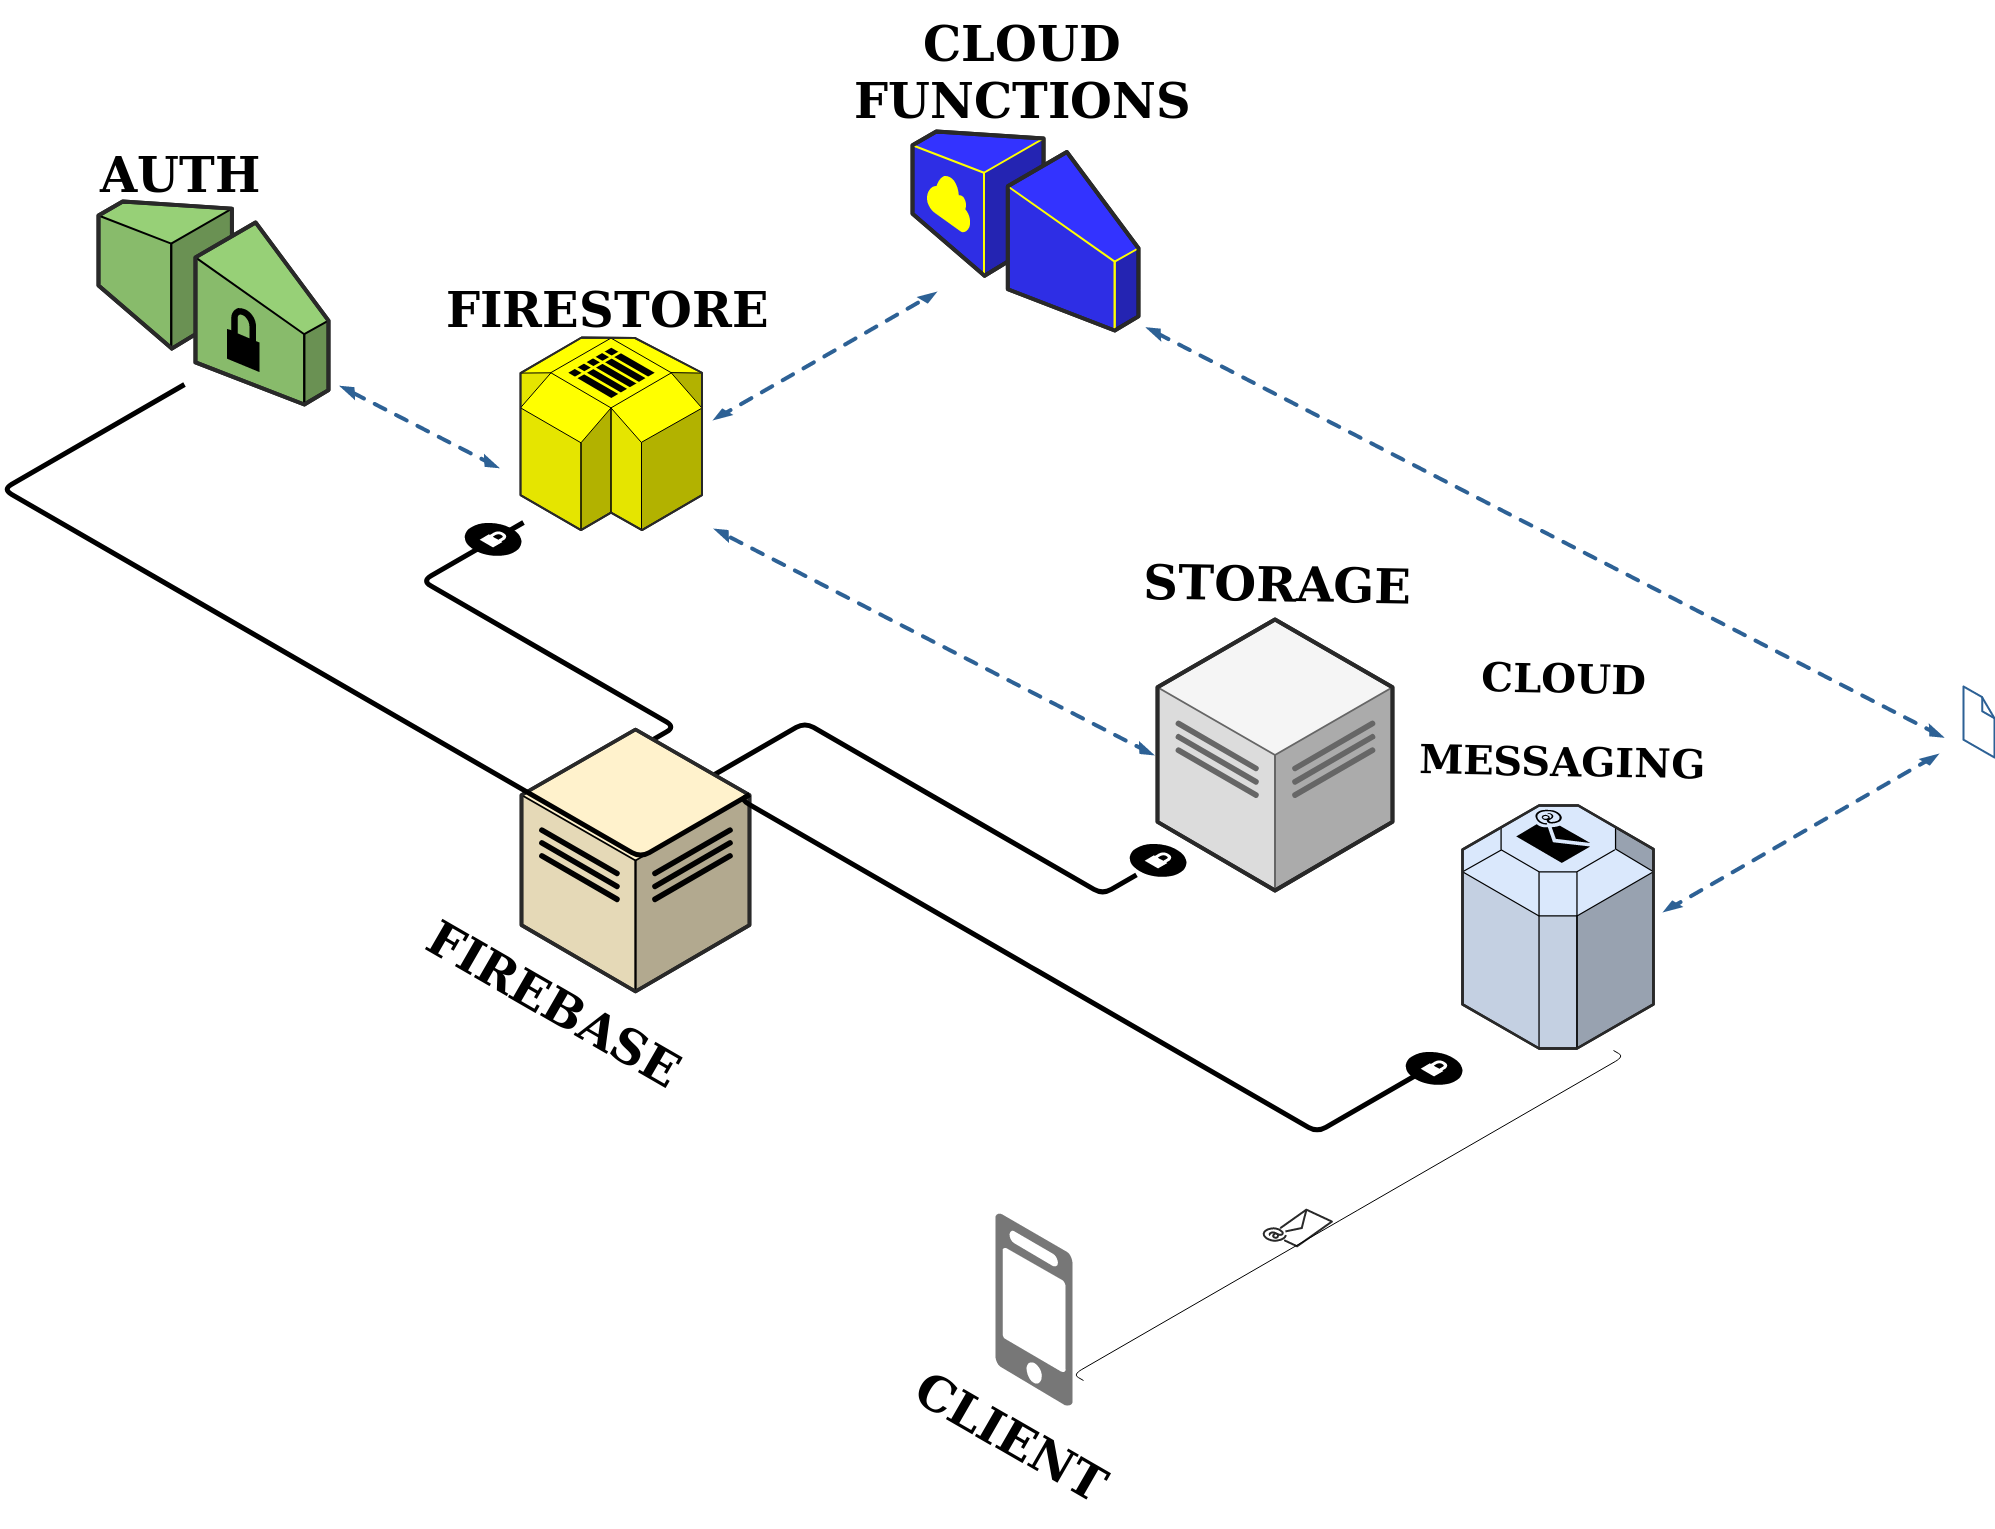
\includegraphics[width=0.7\textwidth]{immagini/server_arch.png}
  \caption{Server Architettura}\label{fig:Architettura Server}
\end{figure}


\section{Model View Presenter}                 %crea la sezione
MVP (Model View Presenter) \'e un pattern architetturale utilizzato per l'organizzazione strutturale di un progetto, in modo da trarne vantaggio in termini di prestazioni, leggibilit\'a e modularit\'a del codice.\\
La sua caratteristica principale \'e quella di separare il livello di presentazione dalla logica, in modo che tutto ci\'o che riguarda l'interazione dell'utente con l'interfaccia sia separato da come vengono rappresentati i dati.\\
Il pattern MVP deriva dal pattern MVC (Model View Controller), che ha 3 concetti base, che lo definiscono:

\begin{enumerate}
\item Model: Il modello dei dati da visualizzare
\item View: L'interfaccia utente che visualizza i dati
\item Controller: Controlla l'interazione tra Model e View
\end{enumerate}

La principale differenza tra i due pattern \'e che il Presenter del MVP gestisce la logica tra la View e il Model, e la sua implementazione permette di gestire l'interfaccia utente ma soprattutto rendere pi\'u comoda l'interazione tra interfaccia utente e i dati.\\


Come il pattern MVC, anche il pattern MVP permette di rendere le View indipendenti dalla gestione dei dati, dividendo la logica dell' applicazione in tre livelli distinti, livelli che possono essere testati separatamente.\\
La possibilit\'a di poter testare i livelli separatamente \'e una delle caratteristiche del MVP.\@


\begin{enumerate}
\item Model: Il modello \'e un' interfaccia che definisce i dati da visualizzare.
\item View: La View \'e un' interfaccia passiva che visualizza i dati (il modello) e instrada i comandi utente (eventi) al Presenter per agire su tali dati.
\item Presenter: Il Presenter agisce sul modello e sulla vista. Recupera i dati dai repository (il modello) e li formatta per la visualizzazione nella vista.
\end{enumerate}

\begin{figure}[!h]
  \centering
  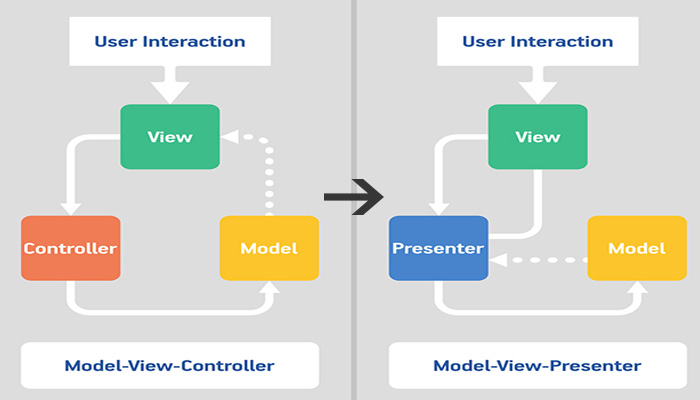
\includegraphics[width=0.65\textwidth]{immagini/mvc-vs-mvp.jpg}
  \caption{MVC vs MVP.}\label{fig:MVC vs MVP}
\end{figure}

\newpage


\subsection{Model}
Il Model \'e un'interfaccia dedicata all'acceso dei dati di un'applicazione, si occupa quindi di fornire un'astrazione del modello dei dati presenti nel database.\\
Il Model oltre a contenere la struttura dei dati da visualizzare si occupa anche di fornire una buona astrazione dei dati presenti nel database, modificando, aggiungendo e separando alcuni dei dati, in modo da rendere l'accesso e la visualizzazione dei dati pi\'u semplice per gli altri due componenti del pattern (View, Presenter).\\
Un esempio potrebbe essere il seguente:
Il database contiene una tabella con due tipi di dato:

\begin{enumerate}
\item \textbf{Nome}: String
\item \textbf{DataDiNascita}: Date
\end{enumerate}

Quando il programma ricever\'a i dati dal database in un qualsiasi formato( Map, Json, Array..) il Model selezionerà i dati in base alla definizione data dal programmatore trasformando il risultato del database in un oggetto.
Questo oggetto oltre a conserare le due informazioni ricevute dal database (Nome, DataDiNascita) potr'\a contenere ance informazioni aggiuntive inserite dal Model per facilitare l'uso e la manipolazione degli altri due componeti.
In questo caso il modello potrebbe creare il nuovo campo "et\'a" facendo una semplice sottrazione fra due date, quella attuale e la data di nascita dell'utente.

\begin{enumerate}
\item \textbf{Nome}: String
\item \textbf{DataDiNascita}: Date
\item \textbf{Et\'a}: Int
\end{enumerate}

%https://medium.com/@cervonefrancesco/model-view-presenter-android-guidelines-94970b430ddf

\subsection{View}
La View \'e un' interfaccia che definisce cosa deve implementare il Presenter, affinch\'e possa interagire con l'interfaccia utente.\\
La View interagisce con il Presenter per visualizzare i dati e notifica al Presenter le azioni che compie l'utente nell'interfaccia.\\
La View pu\'o essere implementata da un Activity, un Fragment, o un widget Android, che contengono ProgressBar, TextView, RecyclerView o altri elementi che necessitano di essere aggiornarnati in base a qualche azione dell'utente o cambiamento nel server.\\
Una delle problematiche riscontrare durante il testing delle view in Android sono causate della complessità del framework.Per risolvere questo problema, attraverso l'utilizzo del pattern MVP è possibile implementare una Passive View( modello di vista passivo).
La sua implementazione riduce al minimo la quantità di logica implementata nella vista.
Ad esempio, se si dispone di un modulo username/password e di un pulsante "Invia", non si scrive la logica di validazione all' interno della View ma all' interno del Presenter. La View infatti dovrebbe solo contenere il nome utente e la password e inviarli al Presenter.



\subsection{Presenter}
Il Presenter \'e il mediatore tra il Model e la View e si occupa di  recuperare i dati dal Model, formattarli e passarli alla View, ma a differenza del pattern MVC, decide anche cosa succede quando si interagisce con la View reagendo alle interazioni dell'utente.\\
Il Presenter per facilitare il testing deve cercare di non dipendere minimamente da Android, ma contenere solo metodi e dipendente Java, senza l'utilizzo del "Context" ad esempio, questo permetter\'a di scrivere i test per il Presenter senza l'utilizzo di un emulatore Android.\\
Come detto in precedenza  il Presenter deve dipendere dall' interfaccia View e non direttamente dall' Activity o Fragment, in questo modo si tengono separati il Presenter e l'Activity rispettando la D dei principi SOLID:"Dipendi dalle astensioni. Non dipendere dalle concrezioni"\\





%%%%%%%%%%%%%%%%%%%%%%%%%%%%%%%%%%%%%%%%%non numera l'ultima pagina sinistra
\clearpage{\pagestyle{empty}\cleardoublepage}

%%%%%%%%%%%%%%%%%%%%%%%%%%%%%%%%%%%%%%%%%imposta l'intestazione di pagina
\renewcommand{\chaptermark}[1]{\markright{\thechapter \ #1}{}}
\lhead[\fancyplain{}{\bfseries\thepage}]{\fancyplain{}{\bfseries\rightmark}}



\appendix                               %imposta le appendici
\chapter{Prima Appendice}               %crea l'appendice
In questa Appendice non si \`e utilizzato il comando:\\
%%%%%%%%%%%%%%%%%%%%%%%%%%%%%%%%%%%%%%%%%\verb"" � equivalente all'
                                        %   ambiente verbatim,
                                        %   ma si utilizza all'interno
                                        %   di un discorso.
\verb"\clearpage{\pagestyle{empty}\cleardoublepage}", ed infatti
l'ultima pagina 8 ha l'intestazione con il numero di pagina in
alto.

%%%%%%%%%%%%%%%%%%%%%%%%%%%%%%%%%%%%%%%%%per fare le conclusioni
\chapter*{Conclusioni}
%%%%%%%%%%%%%%%%%%%%%%%%%%%%%%%%%%%%%%%%%imposta l'intestazione di pagina
\rhead[\fancyplain{}{\bfseries
Conclusioni}]{\fancyplain{}{\bfseries\thepage}}
\lhead[\fancyplain{}{\bfseries\thepage}]{\fancyplain{}{\bfseries
Conclusioni}}
\addcontentsline{toc}{chapter}{Conclusioni}

Lo stato dell'arte al momento in cui si scrive \`e un'applicazione in grado di gestire eventi, commissioni da svolgere, spese condivise e chat, attraverso l'utilizzo di un database aggiornato e consultabile in tempo reale, e la possibilità di gestire e creare le notifiche non appena avviene un cambiamento su di esso.\\
L'applicazione pur garantendo l'uso quotidiano delle funzionalità può essere ulteriormente migliorata, aggiungendo funzionalità, rendendola più stabile e riscriverla anche per la piattaforma iOS. Alcune idee in fase di sviluppo che verrano implementante sono le seguenti:
\begin{itemize}
  \item Chat di messaggistica istantanea anche fra i singoli componenti del gruppo
  \item Migliore flessibilità e funzionalità nella gestione degli eventi
  \item Nuovi informazioni inseribili all'interno di una spesa o commissione
  \item Permettere all'untente di partecipare a più di un gruppo contemporaneamente
  \item Scrivere l'applicazione per iOS utilizzando il linguaggio Swift
\end{itemize}
Attualmente il codice dell'applicazione è presente su Gitlab\footnote{http://gitlab.com/}, in una repository privata, non appena l'applicazione sarà considerata stabile e con le funzionalità desiderate, verrà resa pubblica.\\
L'applicazione è stata scritta utilizzando il linguaggio di programmazione Kotlin, a differenza del linguaggio Java solitamente utilizzato nello sviluppo di applicazioni mobili Android.\\ L'utilizzo di Kotlin come linguaggio per lo sviluppo dell'applicazione mi ha permesso di documentarmi sui nuovi concetti introdotti dal linguaggio e porlo a confronto con Java.\\
I risultati ricavabili dal confronto effettuato, sono stati significativi soprattutto per quanto riguarda le linee di codice, infatti prendendo in considerazione una parte del progetto scritta in Kotlin e confrontato con la relativa parte del progetto precedentemente scritta in Java, alcuni file che in Java richiedevono 140 linee di codice in Kotlin la stessa logica venica implementata in circa 80 linee per quanto.

riguarda le prestazioni e la memoria utilizzata invece si hanno valori trascurabili.\\



\begin{figure}[!hb]
  \centering
  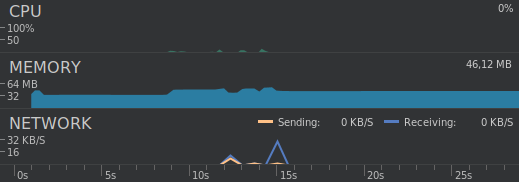
\includegraphics[width=0.8\textwidth]{immagini/app_java_memory_graph.png}
  \caption{Server Architettura}\label{fig:Android Studio }
\end{figure}

\begin{figure}[!hb]
  \centering
  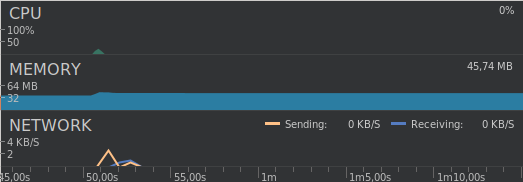
\includegraphics[width=0.8\textwidth]{immagini/app_kotlin_memory_graph.png}
  \caption{Server Architettura}\label{fig:Android Studio }
\end{figure}





\clearpage{\pagestyle{empty}\cleardoublepage}

%

\begin{thebibliography}{9}

\bibitem{latexcompanion}
Massimo Carli
\textit{Android 6. Guida per lo sviluppatore}.
Apogeo, 2016.

\bibitem{latexcompanion}
Stephen Samuel, Stefan Bocutiu
\textit{Programming Kotlin}.
Packtpub, 2017.

\bibitem{latexcompanion}
 Miloš Vasić
 \textit{Mastering Android Development with Kotlin}.
Packtpub, 2017.


\bibitem{latexcompanion}
Ronak K. Panchal,Akshay K. Patel \textit{A comparative study: Java Vs kotlin Programming in Android}.
International Journal of Innovative Trends in Engineering and Research, 2016.

\bibitem{ReactiveX}
ReactiveX documentation
\\\texttt{http://reactivex.io/documentation}

\bibitem{Android Developer }
Google Android Developer Documentation
\\\texttt{https://developer.android.com}

\bibitem{Firebase}
Google Firebase Documentation
\\\texttt{https://firebase.google.com/docs/}

\bibitem{Google I/O}
Google I/O - 2017
\\\texttt{https://events.google.com/io/}

\bibitem{Kotlin Lang}
Kotlin Language Documentation
\\\texttt{https://kotlinlang.org/docs/kotlin-docs.pdf}

\bibitem{Java Docs}
Oracle Java Documentation
\\\texttt{https://docs.oracle.com/}

\bibitem{Xamarin Guides}
Xamarin Android Google services guides
\\\texttt{https://developer.xamarin.com/guides/android/data-and-cloud-services/}

\bibitem{FirebaseUI-Android}
Libreria per la gestione dei servizi Firebase
\\\texttt{https://github.com/firebase/FirebaseUI-Android}

\bibitem{RxJava}
Libreria di supporto per la programmazione reattiva su Java
\\\texttt{https://github.com/ReactiveX/RxJava}

\bibitem{RxKotlin}
Libreria di supporto per la programmazione reattiva su Kotlin
\\\texttt{https://github.com/ReactiveX/RxAndroid}

\bibitem{RxAndroid}
Libreria di supporto per la programmazione reattiva su Android
\\\texttt{https://github.com/ReactiveX/RxKotlin}

\bibitem{BottomNavigationViewEx}
Libreria di supporto per il Widget del menu di navigazione
\\\texttt{https://github.com/ittianyu/BottomNavigationViewEx}

\bibitem{Welcome Android}
Libreria di supporto per mostrare pagine di presentazione e introduzione iniziali
\\\texttt{https://github.com/stephentuso/welcome-android}

\bibitem{MoneyEditText}
Libreria di supporto per il widget che consente di indicare l'ammontare di una spesa
\\\texttt{https://github.com/shuhart/MoneyEditText}

\bibitem{LoadingButtonAndroid }
Libreria di supporto per il widget che trasforma un Button in una barra di caricamento
\\\texttt{https://github.com/leandroBorgesFerreira/LoadingButtonAndroid}

\bibitem{Glide}
Libreria di supporto per la gestione delle immagini con funzionalità di caching
\\\texttt{https://github.com/bumptech/glide}

\bibitem{CircleImageView}
Libreria di supporto per visualizzare immagini con un bordo circolare
\\\texttt{https://github.com/hdodenhof/CircleImageView}

\bibitem{SublimePicker}
Libreria di supporto per la selezione di una data da un calendario personalizzabile
\\\texttt{https://github.com/vikramkakkar/SublimePicker/}

\bibitem{ImagePicker}
Libreria di supporto per selezionare un'immagine dalla galleria del dispositivo
\\\texttt{https://github.com/Mariovc/ImagePicker}

\bibitem{facebook Android SDK}
Libreria di supporto per l'accesso tramite il social network Facebook
\\\texttt{https://github.com/facebook/facebook-android-sdk}


\bibitem{Firebase Command Line Tools}
Tool a linea di comando per gestire i servizi Firebase
\\\texttt{https://github.com/facebook/facebook-android-sdk}


\bibitem{Firebase SDK for Cloud Functions}
Libreria di supporto per l'utilizzo del servizio Firebase Cloud Functions
\\\texttt{https://github.com/firebase/firebase-functions}




\end{thebibliography}




\chapter*{Ringraziamenti}
\thispagestyle{empty}
Un ringraziamento speciale alla mia famiglia che mi ha sempre sostenuto.


\end{document}
